\begin{mainquestion}{solderpaste}{Solderpasted}

\begin{center}
    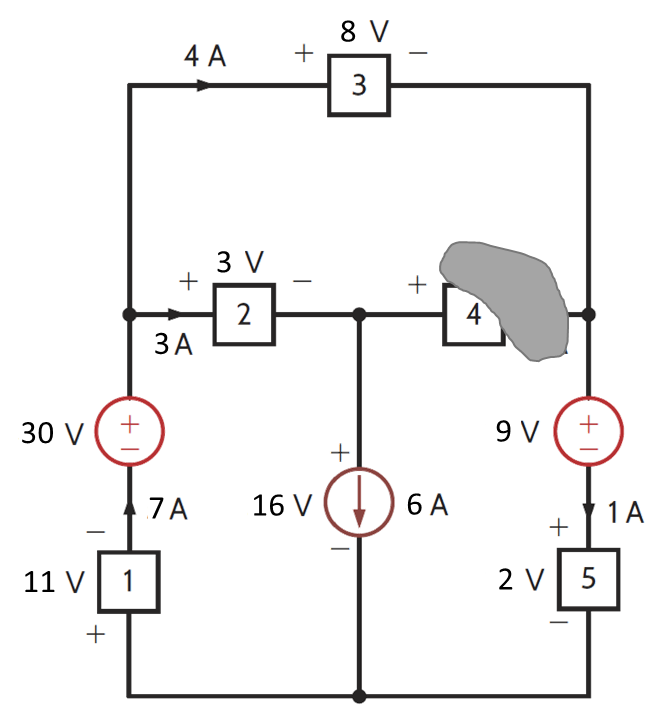
\includegraphics[]{schematic.png}
\end{center}

% =========================================================
\begin{partquestion}{powerall}
{Calculate the power absorbed or supplied by each network element (including sources) except for element \#4, which appears to have some solder paste smeared over its label.}

\begin{answer}
The power is simply P=IV for each element.  Here we follow the passive sign convention which states that the power will be negative if the current as drawn flows into the cathode, and will be positive if the current as drawn flows into the anode.  If the power is negative, the element is supplying power.  If the power is negative, the element is absorbing power.

\begin{table}[htbp]
\centering
\label{tab:power_balance}
\begin{tabular}{|c | c|  c|}
\hline
\textbf{Element} & \textbf{Power (\si{\watt})} & \textbf{Absorbing / Supplying} \\
\hline
30 V source & (-30)(7) = -210 & Supplying \\ \hline
9 V source & (9)(1) = 9 & Absorbing \\ \hline
6 A source & (16)(6) = 96 & Absorbing \\ \hline
1 & (11)(7) = 77 & Absorbing \\ \hline
2 & (3)(3) = 9 & Absorbing \\ \hline
3 & (8)(4) = 32 & Absorbing \\ \hline
4 & ??? & ???  \\ \hline
5 & (2)(1) = 2 & Absorbing \\ \hline
\end{tabular}
\end{table}

\end{answer}
\end{partquestion}

% =========================================================
\begin{partquestion}{powersingle}
{Without direct knowledge of the current and voltage for element \#4, can you find the power absorbed or supplied by element \#4?  If so, what is it, and if not, why not?}
\label{prob:solderpaste:power}

\begin{answer}
Absolutely, we can use Tellegen’s theorem which says the sum of all power absorbed or supplied in a circuit must be zero.  Adding up the powers known, we have:
\[
P_{\text{total}}=-210+9+96+77+9+32+P_4+2=0
\]
Solving for $P_4$ gives $P_4=\qty{-15}{\watt}$, so the element is supplying power to the circuit. 

\end{answer}
\end{partquestion}

% =========================================================
\begin{partquestion}{vasingle}
{Can you determine the current and/or voltage through element \#3?  If so, what are the values, and if not, why not?}

\begin{answer}
Once again, we can certainly do this using KCL or KVL.  Let’s choose to employ KCL.  We can readily see that the current flowing into element 4 from the right is 4 – 1 = 3 A.  This matches our expectation, since this is the cathode side and we expect a positive current going into the negative terminal of the element to yield a negative power, as we saw in part (\cref{prob:solderpaste:power}).  The voltage is then: $V=\frac{-P}{I}=\frac{15}{3}=5\mathrm{\ V}.$
\end{answer}
\end{partquestion}

\end{mainquestion}